%%%%%%%%%%%%%%%%%%%%%%%%%%%%%%%%%%%%%%%%%
% Lachaise Assignment
% LaTeX Template
% Version 1.0 (26/6/2018)
%
% This template originates from:
% http://www.LaTeXTemplates.com
%
% Authors:
% Marion Lachaise & François Févotte
% Vel (vel@LaTeXTemplates.com)
%
% License:
% CC BY-NC-SA 3.0 (http://creativecommons.org/licenses/by-nc-sa/3.0/)
% 
%%%%%%%%%%%%%%%%%%%%%%%%%%%%%%%%%%%%%%%%%

%----------------------------------------------------------------------------------------
%	PACKAGES AND OTHER DOCUMENT CONFIGURATIONS
%----------------------------------------------------------------------------------------

\documentclass{article}

%%%%%%%%%%%%%%%%%%%%%%%%%%%%%%%%%%%%%%%%%
% Lachaise Assignment
% Structure Specification File
% Version 1.0 (26/6/2018)
%
% This template originates from:
% http://www.LaTeXTemplates.com
%
% Authors:
% Marion Lachaise & François Févotte
% Vel (vel@LaTeXTemplates.com)
%
% License:
% CC BY-NC-SA 3.0 (http://creativecommons.org/licenses/by-nc-sa/3.0/)
% 
%%%%%%%%%%%%%%%%%%%%%%%%%%%%%%%%%%%%%%%%%

%----------------------------------------------------------------------------------------
%	PACKAGES AND OTHER DOCUMENT CONFIGURATIONS
%----------------------------------------------------------------------------------------

\usepackage{amsmath,amsfonts,stmaryrd,amssymb} % Math packages

\usepackage{enumerate} % Custom item numbers for enumerations

\usepackage[ruled]{algorithm2e} % Algorithms

\usepackage[framemethod=tikz]{mdframed} % Allows defining custom boxed/framed environments

\usepackage{listings} % File listings, with syntax highlighting
\lstset{
	basicstyle=\ttfamily, % Typeset listings in monospace font
}

%----------------------------------------------------------------------------------------
%	DOCUMENT MARGINS
%----------------------------------------------------------------------------------------

\usepackage{geometry} % Required for adjusting page dimensions and margins

\geometry{
	paper=a4paper, % Paper size, change to letterpaper for US letter size
	top=2.5cm, % Top margin
	bottom=3cm, % Bottom margin
	left=2.5cm, % Left margin
	right=2.5cm, % Right margin
	headheight=14pt, % Header height
	footskip=1.5cm, % Space from the bottom margin to the baseline of the footer
	headsep=1.2cm, % Space from the top margin to the baseline of the header
	%showframe, % Uncomment to show how the type block is set on the page
}

%----------------------------------------------------------------------------------------
%	FONTS
%----------------------------------------------------------------------------------------

\usepackage[utf8]{inputenc} % Required for inputting international characters
\usepackage[T1]{fontenc} % Output font encoding for international characters

\usepackage{XCharter} % Use the XCharter fonts

%----------------------------------------------------------------------------------------
%	COMMAND LINE ENVIRONMENT
%----------------------------------------------------------------------------------------

% Usage:
% \begin{commandline}
%	\begin{verbatim}
%		$ ls
%		
%		Applications	Desktop	...
%	\end{verbatim}
% \end{commandline}

\mdfdefinestyle{commandline}{
	leftmargin=10pt,
	rightmargin=10pt,
	innerleftmargin=15pt,
	middlelinecolor=black!50!white,
	middlelinewidth=2pt,
	frametitlerule=false,
	backgroundcolor=black!5!white,
	frametitle={Command Line},
	frametitlefont={\normalfont\sffamily\color{white}\hspace{-1em}},
	frametitlebackgroundcolor=black!50!white,
	nobreak,
}

% Define a custom environment for command-line snapshots
\newenvironment{commandline}{
	\medskip
	\begin{mdframed}[style=commandline]
}{
	\end{mdframed}
	\medskip
}

%----------------------------------------------------------------------------------------
%	FILE CONTENTS ENVIRONMENT
%----------------------------------------------------------------------------------------

% Usage:
% \begin{file}[optional filename, defaults to "File"]
%	File contents, for example, with a listings environment
% \end{file}

\mdfdefinestyle{file}{
	innertopmargin=1.6\baselineskip,
	innerbottommargin=0.8\baselineskip,
	topline=false, bottomline=false,
	leftline=false, rightline=false,
	leftmargin=0.5cm,
	rightmargin=0.5cm,
	singleextra={%
		\draw[fill=black!10!white](P)++(0,-1.2em)rectangle(P-|O);
		\node[anchor=north west]
		at(P-|O){\ttfamily\mdfilename};
		%
		\def\l{3em}
		\draw(O-|P)++(-\l,0)--++(\l,\l)--(P)--(P-|O)--(O)--cycle;
		\draw(O-|P)++(-\l,0)--++(0,\l)--++(\l,0);
	},
	nobreak,
}

% Define a custom environment for file contents
\newenvironment{file}[1][File]{ % Set the default filename to "File"
	\medskip
	\newcommand{\mdfilename}{#1}
	\begin{mdframed}[style=file]
}{
	\end{mdframed}
	\medskip
}

%----------------------------------------------------------------------------------------
%	NUMBERED QUESTIONS ENVIRONMENT
%----------------------------------------------------------------------------------------

% Usage:
% \begin{question}[optional title]
%	Question contents
% \end{question}

\mdfdefinestyle{question}{
	innertopmargin=1.2\baselineskip,
	innerbottommargin=0.8\baselineskip,
	roundcorner=5pt,
	nobreak,
	singleextra={%
		\draw(P-|O)node[xshift=1em,anchor=west,fill=white,draw,rounded corners=5pt]{%
		Question \theQuestion\questionTitle};
	},
}

\newcounter{Question} % Stores the current question number that gets iterated with each new question

% Define a custom environment for numbered questions
\newenvironment{question}[1][\unskip]{
	\bigskip
	\stepcounter{Question}
	\newcommand{\questionTitle}{~#1}
	\begin{mdframed}[style=question]
}{
	\end{mdframed}
	\medskip
}

%----------------------------------------------------------------------------------------
%	WARNING TEXT ENVIRONMENT
%----------------------------------------------------------------------------------------

% Usage:
% \begin{warn}[optional title, defaults to "Warning:"]
%	Contents
% \end{warn}

\mdfdefinestyle{warning}{
	topline=false, bottomline=false,
	leftline=false, rightline=false,
	nobreak,
	singleextra={%
		\draw(P-|O)++(-0.5em,0)node(tmp1){};
		\draw(P-|O)++(0.5em,0)node(tmp2){};
		\fill[black,rotate around={45:(P-|O)}](tmp1)rectangle(tmp2);
		\node at(P-|O){\color{white}\scriptsize\bf !};
		\draw[very thick](P-|O)++(0,-1em)--(O);%--(O-|P);
	}
}

% Define a custom environment for warning text
\newenvironment{warn}[1][Warning:]{ % Set the default warning to "Warning:"
	\medskip
	\begin{mdframed}[style=warning]
		\noindent{\textbf{#1}}
}{
	\end{mdframed}
}

%----------------------------------------------------------------------------------------
%	INFORMATION ENVIRONMENT
%----------------------------------------------------------------------------------------

% Usage:
% \begin{info}[optional title, defaults to "Info:"]
% 	contents
% 	\end{info}

\mdfdefinestyle{info}{%
	topline=false, bottomline=false,
	leftline=false, rightline=false,
	nobreak,
	singleextra={%
		\fill[black](P-|O)circle[radius=0.4em];
		\node at(P-|O){\color{white}\scriptsize\bf i};
		\draw[very thick](P-|O)++(0,-0.8em)--(O);%--(O-|P);
	}
}

% Define a custom environment for information
\newenvironment{info}[1][Info:]{ % Set the default title to "Info:"
	\medskip
	\begin{mdframed}[style=info]
		\noindent{\textbf{#1}}
}{
	\end{mdframed}
}
 % Include the file specifying the document structure and custom commands

%----------------------------------------------------------------------------------------
%	ASSIGNMENT INFORMATION
%----------------------------------------------------------------------------------------

\title{Operational Statistics for SAR Imagery Course Assignment} % Title of the assignment

\author{jun li\\ \texttt{19171213765}} % Author name and email address

\date{Xidian University --- \today} % University, school and/or department name(s) and a date

%----------------------------------------------------------------------------------------

\begin{document}
	
	\maketitle % Print the title
	
	%----------------------------------------------------------------------------------------
	%	INTRODUCTION
	%----------------------------------------------------------------------------------------
	
	\section*{Basic model function} % Unnumbered section
	\par During the class, we first studied several deferent probability distributions which is used to fitting SAR image statistical model.  We try to draw the distribution of Exponential. The function is:
	% Math equation/formula
	\begin{equation}
	\mathop {f(x)=\frac{1}{\theta} e^\frac{-x}{\theta}}
	\end{equation}
	\par I used ggplot2 to draw this equation and then I converted that to log10. The plot is shown as Figure 1.
	\begin{figure}[h] % [h] forces the figure to be output where it is defined in the code (it suppresses floating)
		\centering
		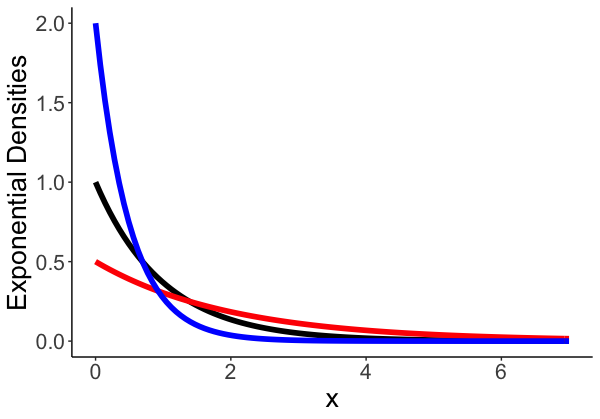
\includegraphics[width=2in]{picture/exp_dens.png} % Example image
		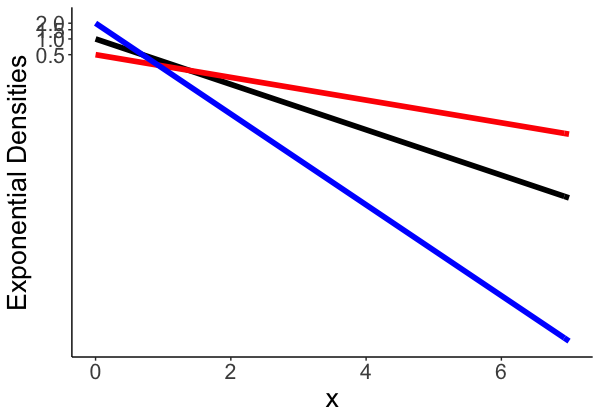
\includegraphics[width=2in]{picture/exp_dens_log.png}
		\caption{Exponential distribution(left) and Exponential distribution in log10(right)}
	\end{figure}
	\par Except this, we plot the distribution of Gamma. Function is:
	\begin{equation}
	\mathop {f(x,\beta,\alpha)=\frac{\beta^\alpha}{\Gamma ( \alpha ) } x^{\alpha-1} e^{-\beta x}}
	\end{equation}
	\par Then I used ggplot2 to draw this equation and then I converted that to log10, too. The plot is shown as Figure 2.
	\begin{figure}[h] % [h] forces the figure to be output where it is defined in the code (it suppresses floating)
		\centering
		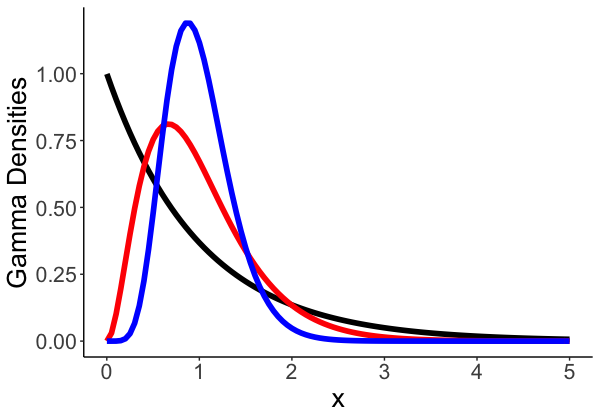
\includegraphics[width=2in]{picture/gamma_dis.png} % Example image
		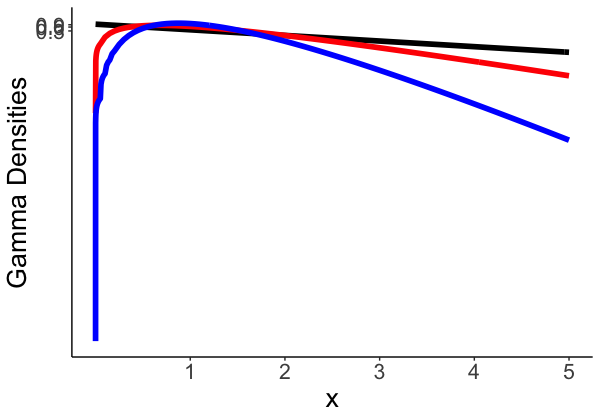
\includegraphics[width=2in]{picture/gamma_log.png}
		\caption{Gamma distribution(left) and Gamma distribution in log10(right)}
	\end{figure}
    
    \par Besides plot them by ggplot2. All of these function were first drawing by my usual tool MATLAB. And the figures are not showing here.
	
	\section*{ SAR Image Analysis} % Numbered section
	According to the assignment, I've taken a portion of the image from figure 3.4, which is in the lower left corner showing the forest.  The original image and the captured image are shown below: 
	
	\begin{figure}[h] % [h] forces the figure to be output where it is defined in the code (it suppresses floating)
		\centering
		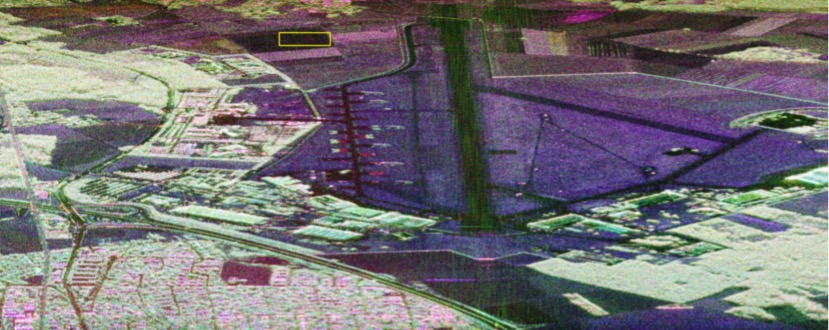
\includegraphics[width=4in]{picture/oripic.png} % Example image
		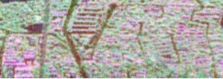
\includegraphics[width=2in]{picture/pic.jpg}
		\caption{Original image(left) and Captured image(right)}
	\end{figure}
	
	\par For the captured image, I use function 'hist'  to process it to be Gray histogram as Figure 4.
	
	\begin{figure}[h] % [h] forces the figure to be output where it is defined in the code (it suppresses floating)
		\centering
		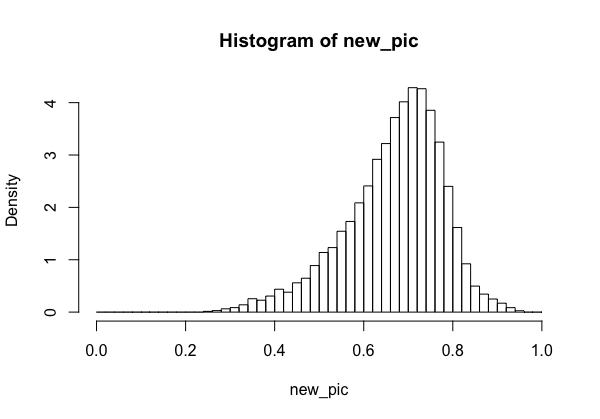
\includegraphics[width=4in]{picture/hist.png} % Example image
		\caption{Gray histogram}
	\end{figure}
	
    \par After gathering the gray histogram, I try to modeling, in other words fitting, the histogram using the aforementioned function. It's obvious that the histogram is following the Gamma distribution. So I selected several different parameters to change the lines' shape in order to fitting the results. I compared the line's fitting outcom with the shape parameter being 3 and the scale parameter being 1/7, 1/8 and 1/9, respective. But in doing this, some problem occured. The maximum value of the histogram is nearly 40 and the fluctuations in the curve are very small and almost invisible because the top value of curve is just about 5 which is small in contrast to the histogram value. To solve this problem, I normalized the histogram but in this circumstance, the curve fit well in the high-light region and fit terriblly in the dark region. At last, I was inspired by my roommate who normalized the histogram to a larger number instead of to 1. By means of this tip, I successfully achieved the analyses. 
    
    \begin{figure}[h] % [h] forces the figure to be output where it is defined in the code (it suppresses floating)
    	\centering
    	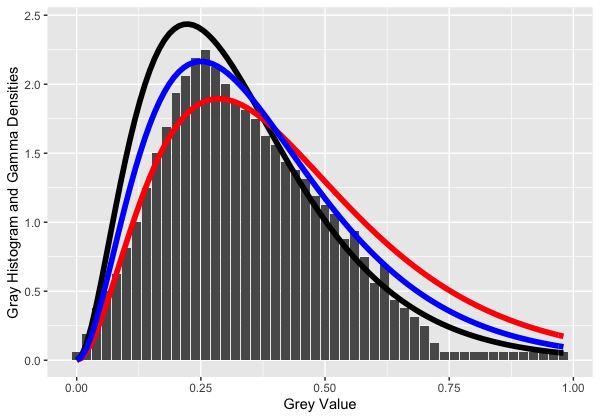
\includegraphics[width=4in]{picture/Rplot.png} % Example image
    	\caption{ Final results}
    \end{figure}

    \begin{warn}[Codes:]
    	The code to process the image is in the file ' SARexc.R '.
    \end{warn}
	% File contents

\end{document}






